\documentclass[12pt, letterpaper]{article}
\usepackage[margin=1in]{geometry}
\usepackage[utf8]{inputenc}
\usepackage{indentfirst}
\usepackage{graphicx}
\usepackage{float}
\usepackage{hanging}
\graphicspath{ {./img/} }
\renewcommand\thesection{\Roman{section}}

\title{A Brief History of Supercomputing}
\author{Zachary M. Mattis}

\begin{document}

\maketitle

\begin{abstract}
Supercomputing is the dynamic field of problem solving that attempts to push the boundaries of size, power, and performance of modern systems in order to solve extremely complex and advanced technical problems via incredible performance standards. Since their creation in the 1960s, engineers have continued to push the limits of supercomputing, creating new machines that were once believed to be impossible. 

\end{abstract}

\section{Introduction}

Since standard computers lie at the backbone of supercomputing, it is extremely necessary to explore the history of traditional computing and how it lead to the supercomputer. Widespread observance of computing began in the late 1940s in response to the rising challenges of World War II. However, British scientist Charles Babbage is credited as inventing the computer in the late 1800s as it is understood and implemented today. Babbage designed the analytic engine, a proposed device featuring a “mill” for conducting arithmetic operations, a “store” for saving information, and programmable punch cards [Hal70]. While Babbage’s machine was not physically built in his lifetime, his accomplishments have become increasingly prevalent today.

Computer scientist Alan Turing is often credited with sparking the age of computation, through his numerous contributions to computer science. Famously, Turing created an electromechanical device known as the Bombe which he used to crack the German Enigma encryption code. President Eisenhower credited his contributions, adding that it possibly shortened the war by nearly two years. This incredible feat began to show the true power of such devices, with the 1950s beginning a new era in computation, based on Turing’s Universal Machine [CD11]. Turing’s contributions would catapult engineering efforts to create super machines, capable of performing record-setting calculations and solving new problems.

\section{History}

Often characterized as the first supercomputer, the Control Data Corporation 6600 was designed in 1964. It was a single processor design capable of 10 million instruction per second [Cer03]. This machine sparked an era of supercomputing defined by Seymour Cray and Cray-derivative architectures. These machines were characterized by a shared memory utilized by multiple processors. These computers utilized a combination of increased processor speed, pipelined instruction set, and increased ISA for vector calculations in order to increase overall performance. Around the 1990s, evolution of these types of systems began to halt as processor speeds began to stall and the number of processors able to access the same memory was limited to a few dozen [SAB17].

Around the mid 1980s, the scalability and cost effectiveness of multiple interconnected high-powered computers was demonstrated and observed. This sparked a new era of supercomputing, abandoned the idea of a single program memory with sequential operation flow. This new idea of distributed memory across separate computers serves as the foundation for the incredibly powerful supercomputers that exist today [SAB17].

Through the technological advancements in supercomputing, researchers have been able to solve unique problems, including mapping of the human genome, quantum mechanics, and climate research.

\section{Modern Supercomputing}

A couple of important characteristics can be observed from the very top supercomputers in the world, as shown in Figure 1. While \textit{Summit} is capable of over 1.5 times the number of operations as \textit{Sunway TaijuLight}, it only has approximately 1/4 the number of cores and consumes 2/3 the power. Very strong conclusions can be drawn from this figure, most notably how the implementation of these vast systems can lead to strikingly different performances. From a naïve perspective, one might assume that a computer with 4 times as many cores would be capable of greater performance. \textit{Summit} proves that just throwing more hardware at a problem will not yield the top performance possible. Additionally, even with this massive underlying architecture, \textit{Summit} is able to operate at a frequency of 3 GHz, twice the frequency of \textit{Sunway TaijuLight}. The distinction between these two systems yields a snapshot into the complexity of the supercomputing world.

\begin{figure}[H]
	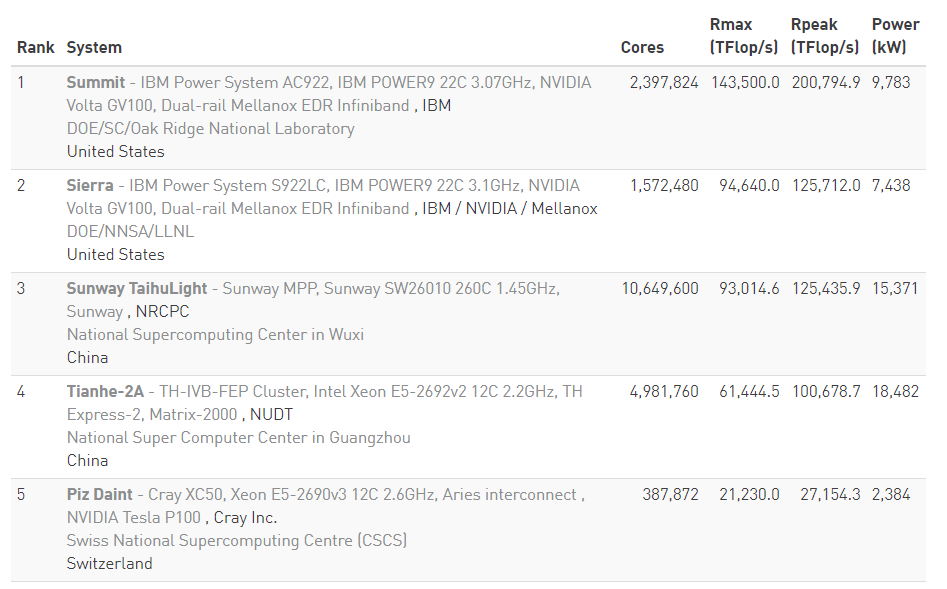
\includegraphics[width=\linewidth]{top5.png}
	\caption{Top 5 Supercomputers (Nov. 2018) [TOP18]}
\end{figure}


Just here in Pittsburgh, there are two major supercomputing centers: the Center for Research Computing (CRC) and the Pittsburgh Supercomputing Center (PSC). A major facet of large-scale computing implementations is in the ease of programmability from a user’s perspective. If a machine is incredibly difficult or complex to use, it may be completely counterproductive to develop and utilize this machine due to the offset of complexity versus performance. Specifically, students at the University of Pittsburgh have the opportunity to utilize the resources of the CRC center and can see their code be compued and carried out on this incredibly advanced hardware. A major shift in the supercomputing paradigm can be accomplished by providing this kind of access to everyday people, similarly to how the very first computers were used. While once used just by governments and large businesses, emerging technology brought this computing availability to the everyday man.

\section{Future of High-Performance Computing}

In order to predict the future of supercomputing, it is equally important to understand the past. Figure 2, from 2010, shows some important events in supercomputing, highlighting the year coupled with the performance in FLOPS. This graph shows a prediction of the exaFLOP by the year 2019, as previous jumps of 3 orders of magnitude took approximately 10-15 years. As previously shown, the current top Supercomputer is still an entire order of magnitude away from reaching this benchmark.

\begin{figure}[H]
	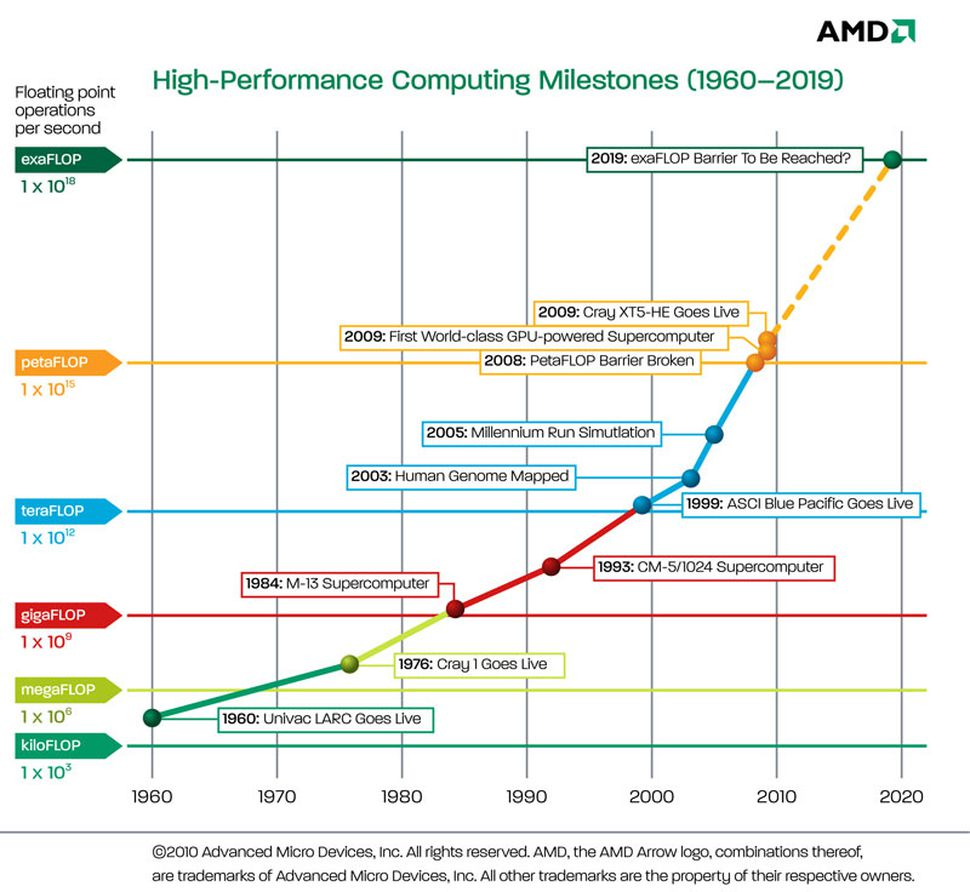
\includegraphics[width=\linewidth]{milestones.jpg}
	\caption{High-Performance Computing Barriers [AMD]}
\end{figure}

This inaccuracy in predication can be attributed to a few factors, including slowing clock speed of microprocessors in regard to the number of transistors, as illustrated in Figure 3. Additionally, Moore’s law is beginning to reach its limit, but not necessarily due to the laws of physics. While it may be possible to create new fabrications of increasingly smaller size from a technical standpoint, it will soon be too economically infeasible as the fabrication technology to create such devices will soon outweigh the value of production [Wal16].

\begin{figure}[H]
	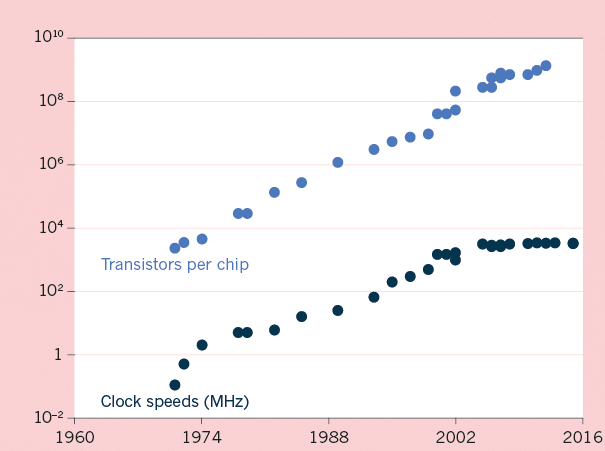
\includegraphics[width=\linewidth]{moore.png}
	\caption{Transistor / Clock Speed Ratio [Wal16]}
\end{figure}

\section{Artificial Intelligence}

From my current understanding of both legacy and modern computing, I strongly believe that Artificial Intelligence will be the major focus of the generations to come and will have revolutionary impact in all areas of life. The invention of a truly conscious AI will completely overthrow modern understandings of computing and push a rapidly shifting way of life not seen since the Industrial Revolution. This type of technology will produce dynamic economic paradigms shifts, as modern careers will quickly become obsolete. Additionally, such a technology could produce massive emotional impacts as we begin to interact with this incredibly vast intelligence.

This computing shift can already be seen today as the top high-performance computing system, \textit{Summit}, was specifically designed and architectured from the ground up for AI applications, including machine learning and neural networks.

\section{Conclusion}

The world of supercomputing dates all the way back to the 1960s, with new technology advancements constantly increasing the performance of these massive machines to what no one could have predicted. In essence, the idea of supercomputing personifies the human spirit. The underlying passion and desire to reach for more, to do things that no one else has done, is implicit in the never-ending quest for more performance.

\section{References}

\begin{hangparas}{.25in}{1}

[Hal70] D. Halacy. Charles Babbage, Father of the Computer. Crowell-Collier Press, New York, 1970.\\

[CD11] J. Copeland, D. Proudfoot. “Alan Turing, Father of the Modern Computer.” Rutherford Journal 4. 2011–2012.\\

[Cer03] P. Ceruzzi. A History of Modern Computing. MIT Press, Cambridge, MA, 2003.\\

[SAB17] T. Sterling, M. Anderson, M. Brodowicz. High Performance Computing: Modern Systems and Practices. Morgan Kaufmann, Burlington, MA, 2017.\\

[TOP18] TOP500. “NOVEMBER 2018.” TOP500. November 2018.\\

[Wal16] M. Waldrop “The chips are down for Moore’s law.” Nature. 09 February 2016.\\

\end{hangparas}

\end{document}
